% !TEX program = lualatex
\documentclass[aspectratio=169,professionalfonts]{beamer}
%------------------------- Preamble (beamer) -------------------------%
%   Require LuaLaTeX + --shell-escape (for minted)                    %
%--------------------------------------------------------------------%
\usepackage[spanish]{babel}

% ---------- Fonts (modern look) ----------
\usepackage{fontspec}
\defaultfontfeatures{Ligatures=TeX, Scale=MatchLowercase}
\setmainfont{Inter}       % Sans‑serif body (install ttf–Inter)
\setsansfont{Inter}
\setmonofont{Fira Code}   % Nice mono for code

% ---------- Theme ----------
\usetheme[
  titleformat=smallcaps,
  numbering=fraction,
  progressbar=frametitle   % thin progress line under the title
]{metropolis}              % modern beamer theme
\metroset{block=fill}      % coloured blocks

% ---------- Colours ----------
\definecolor{clblue}{HTML}{005F9E}
\definecolor{clorange}{HTML}{FF9130}
\definecolor{clgrey}{HTML}{F4F4F4}

% ---------- minted ----------
\usepackage{minted}
\setminted{
  fontsize=\footnotesize,
  autogobble,
  breaklines,
  tabsize=2,
  style=monokai,
  linenos
}

% ---------- Custom boxes (tcolorbox) ----------
\usepackage{tcolorbox}
\tcbuselibrary{skins, breakable}
% Warning box
\newtcolorbox{warnbox}{
  colback=clorange!10,
  colframe=clorange!80!black,
  breakable,
  title={\faWarning\quad Advertencia},
  fonttitle=\bfseries,
  left=2mm, right=2mm, top=1mm, bottom=1mm
}
% Information box
\newtcolorbox{infobox}{
  colback=clblue!5,
  colframe=clblue!60!black,
  breakable,
  title={\faInfoCircle\quad Nota},
  fonttitle=\bfseries,
  left=2mm, right=2mm, top=1mm, bottom=1mm
}

% ---------- Icons ----------
\usepackage{fontawesome5}

% ---------- Misc tweaks ----------
\graphicspath{{figures/}}
\setlength{\parskip}{0.5em}
\addto\extrasspanish{\renewcommand{\contentsname}{Índice}}
%--------------------------------------------------------------------%



\title[ClústerLab • Día 1]{Linux básico y primeros comandos}
\subtitle{Hands--on en Raspberry Pi 5}
\author{Equipo docente ClústerLab}
\date{4 de agosto de 2025}

%--------------------------------------------------------------------
\begin{document}

%------------------------ title -------------------------------------
\begin{frame}[plain]
  \titlepage
\end{frame}

%------------------------ objetivos ---------------------------------
\begin{frame}{Objetivos del curso}
  Una visión muy general de los objetivos de este curso, es que al final del curso podremos tener conocimientos básicos sobre:
  \begin{itemize}
    \item ¿Qué es un \emph{clúster}? ¿Por qué importa?
    \item Configurar un mini-clúster con Raspberry Pi 5.
    \item Fundamentos de Linux, scripting Bash y redes.
    \item Programación paralela (MPI) y proyecto final.
  \end{itemize}
\end{frame}

%------------------------ qué es un clúster -------------------------
\begin{frame}{¿Qué es un clúster?}
  \begin{columns}[T]
    \begin{column}{0.55\textwidth}
      \begin{block}{Definición rápida}
        Conjunto de computadores interconectados que actúan
        como un único recurso de cómputo.
      \end{block}
      \pause
      \begin{itemize}
        \item Alta disponibilidad y escalabilidad \emoji{chart-increasing}
        \item Paralelismo y balanceo de carga
        \item Ciencia de datos, simulaciones, IA.
        \begin{itemize}
          \item Ciencia
          \item Estado
          \item Instituciones Privadas
        \end{itemize}
      \end{itemize}
    \end{column}
    \begin{column}{0.4\textwidth}
      \centering
      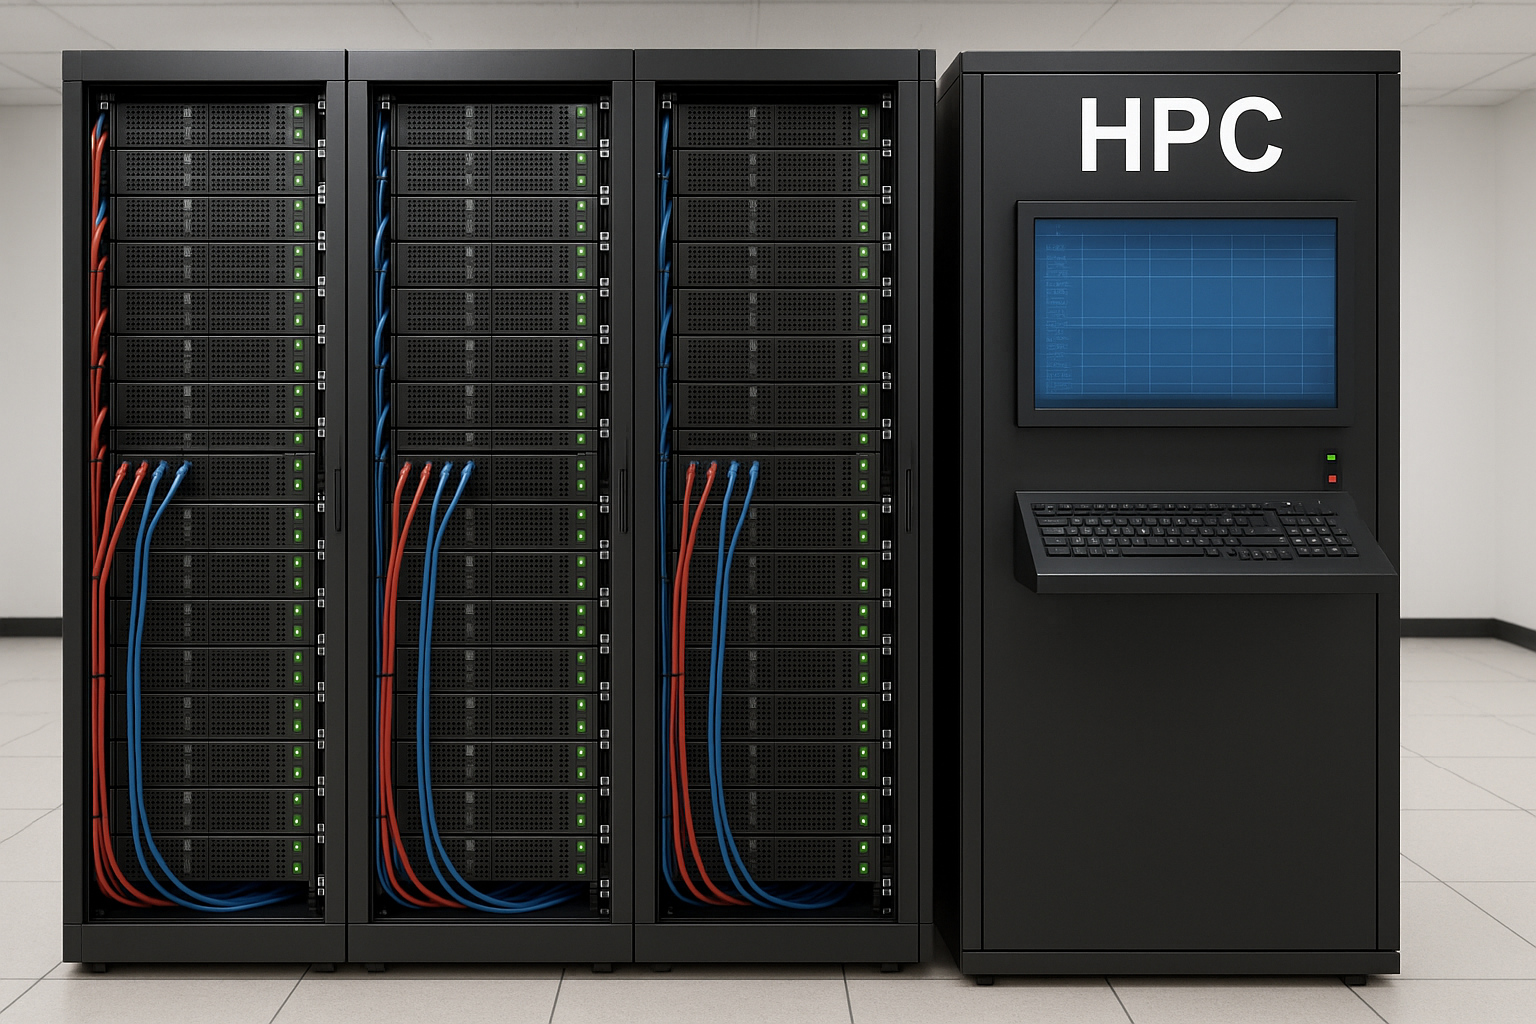
\includegraphics[width=\linewidth]{hpc1.png} % imagen genérica
    \end{column}
  \end{columns}
  \begin{block}{Spolier}
    La segunda semana jugaremos con real-HPC cluster para probar algunas cosas.
  \end{block}
\end{frame}

%------------------------ por qué raspberry -------------------------
\begin{frame}{¿Por qué Raspberry Pi 5?}
  \begin{itemize}
    \item Bajo costo y consumo $\approx$ 5--7 [W] de potencia.
    \item Soporte completo Linux + comunidad enorme.
    \item Perfecta para aprender HPC en \textit{pequeño}.
    \item ¡Quedás listo/a para trabajar en ambientes Linux! \emoji{rocket}
  \end{itemize}
  \vspace{0.4em}
  \centering
  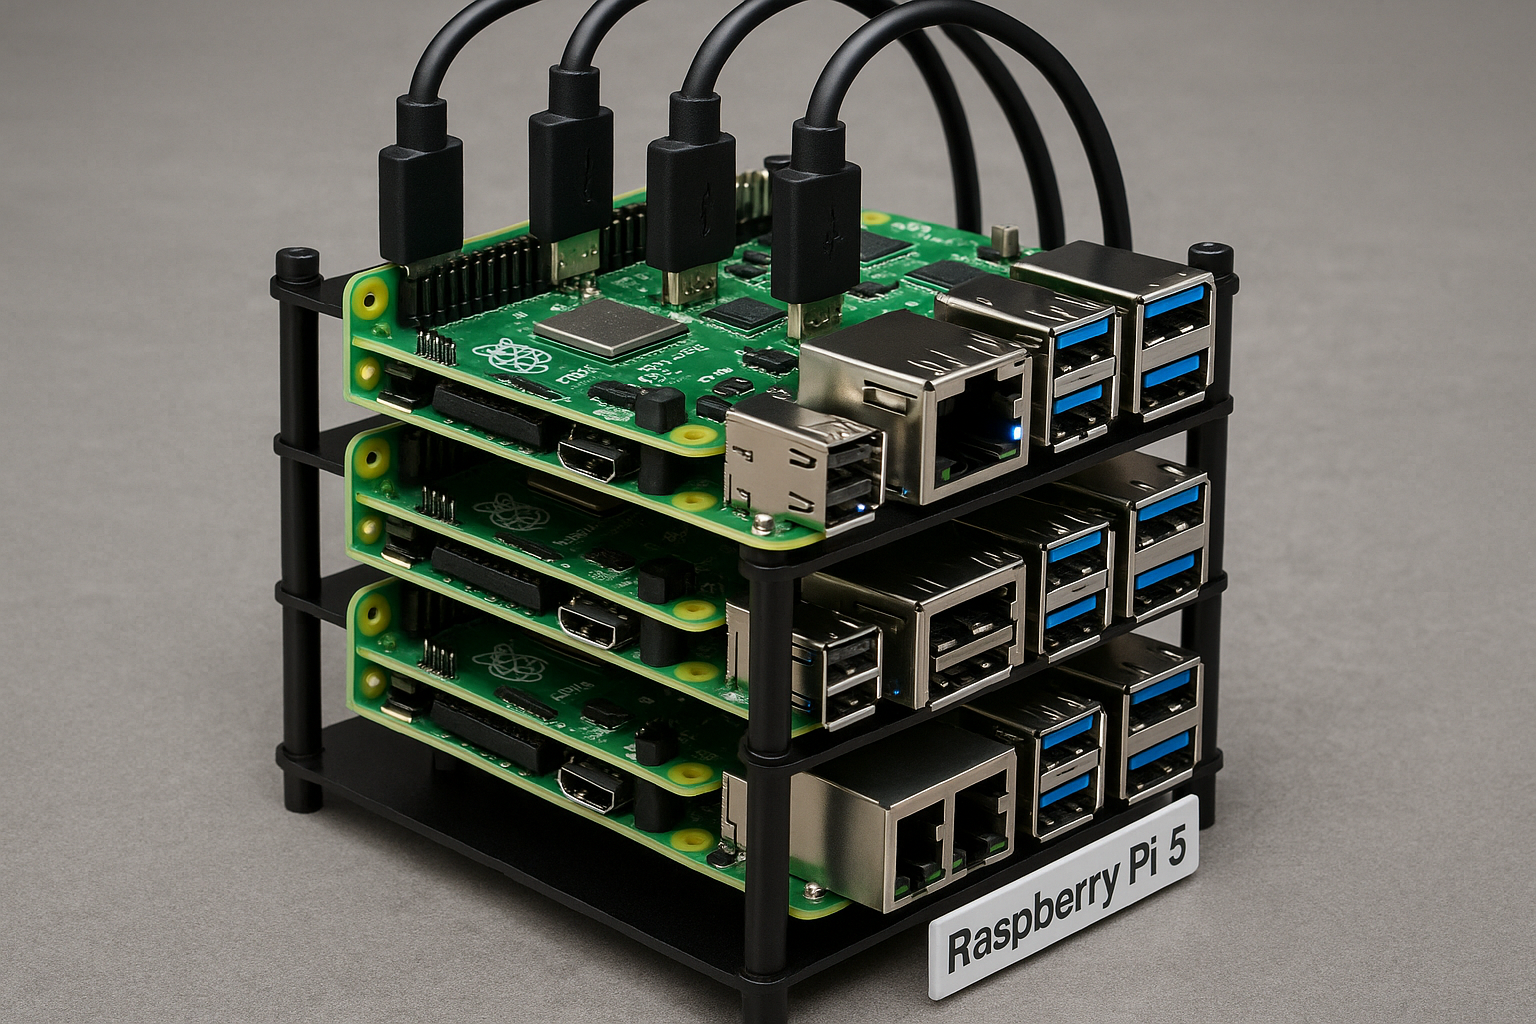
\includegraphics[width=0.5\linewidth]{rpi5-cluster.png} % otra imagen demo
\end{frame}

%------------------------ agenda del día ----------------------------
\begin{frame}{Agenda Día 1 (09:00--13:00)}
  \begin{enumerate}
    \item 09:00 -- 09:15  Bienvenida y motivación.
    \item 09:15 -- 10:30  Encender la Pi + primeros comandos Linux.
    \item 10:45 -- 12:00  Bash I (variables, redirección).
    \item 12:00 -- 13:00  Actividad: árbol de carpetas + backup.
  \end{enumerate}
\end{frame}

%------------------------ requisitos -------------------------------
\begin{frame}[fragile]{Requisitos para hoy}
  \begin{itemize}
    \item computador con acceso a la internet y cliente SSH (Linux/macOS) \textbf{o} WSL 2 en Windows.
    \item Raspberry Pi 5 con SD Card (≥16 GB) y fuente.
    \item Implementos de la Raspberry Pi:
    \begin{itemize}
      \item Cable para Display
      \item Cable re RED + switch
      \item Acceso a Internet por wifi.
    \end{itemize}
  \end{itemize}
  \alert{En Windows es recomendable usar \textbf{WSL 2 + Ubuntu}.}
\end{frame}

%------------------------ WSL --------------------------------------
\begin{frame}{¿Qué es WSL?}
  \begin{itemize}
    \item WSL = Windows Subsystem for Linux.
    \item Permite correr distribuciones Linux (Ubuntu, Debian, etc.) dentro de Windows.
    \item Integra comandos de Linux en Windows, sin usar máquinas virtuales pesadas.
    \item Ideal para aprender Linux, programar, usar herramientas científicas.
  \end{itemize}
\end{frame}

\begin{frame}{Instalar WSL 2 (paso a paso)}
  \begin{enumerate}
    \item Abrir PowerShell como administrador.
    \item Ejecutar: \texttt{wsl --install}
    \item Esperar instalación y reiniciar.
    \item Se instalará Ubuntu por defecto (puede cambiarse).
  \end{enumerate}
\end{frame}

\begin{frame}{Primer inicio de Ubuntu WSL}
  \begin{itemize}
    \item Al abrir Ubuntu WSL, te pedirá crear:
      \begin{itemize}
        \item Nombre de usuario.
        \item Contraseña.
      \end{itemize}
    \item Esto crea tu cuenta en Linux dentro de Windows.
    \item Puedes empezar a usar comandos como: \texttt{ls}, \texttt{pwd}, \texttt{cd}, etc.
  \end{itemize}
\end{frame}


\begin{frame}{Primeros comandos en Linux}
  \begin{itemize}
    \item \texttt{ls} – lista archivos.
    \item \texttt{cd} – cambia de directorio.
    \item \texttt{pwd} – muestra dónde estás.
    \item \texttt{mkdir} – crea carpetas.
    \item \texttt{nano} o \texttt{vim} – editores de texto.
  \end{itemize}
\end{frame}

\begin{frame}{Instalar programas con APT}
  \begin{itemize}
    \item WSL usa el sistema de paquetes de Ubuntu.
    \item Instalar programas con:
      \texttt{\$ sudo apt install nombre\_paquete}
    \item Ejemplo: \texttt{sudo apt install openssh-client}
    \item También puedes instalar: \texttt{git}, \texttt{python3}, \texttt{g++}, etc.
  \end{itemize}
\end{frame}

\begin{frame}{Ver archivos de Windows desde WSL}
  \begin{itemize}
    \item WSL puede ver el sistema de archivos de Windows.
    \item Se encuentra en: \texttt{/mnt/c}, \texttt{/mnt/d}, etc.
    \item Ejemplo:
      \begin{itemize}
        \item \texttt{cd /mnt/c/Users/tu\_usuario/Downloads}
        \item Accedes a tu carpeta de Descargas.
      \end{itemize}
    \item Puedes copiar, mover, editar desde WSL.
  \end{itemize}
\end{frame}

\begin{frame}{Conexión por SSH}
  \begin{itemize}
    \item SSH permite conectarse a otros computadores Linux de forma segura.
    \item Instalamos el cliente con:
      \texttt{sudo apt install openssh-client}
    \item Ejemplo de conexión:
      \texttt{ssh usuario@IP\_remota}
    \item Muy útil para acceder a servidores, Raspberry Pi, etc.
  \end{itemize}
\end{frame}


\begin{frame}{Python y Jupyter en WSL}
  \begin{itemize}
    \item Puedes instalar Python con:
      \texttt{sudo apt install python3 python3-pip}
    \item Luego instalar Jupyter:
      \texttt{pip install notebook}
    \item Ejecutar: \texttt{jupyter notebook}
    \item Abre automáticamente en el navegador de Windows.
  \end{itemize}
\end{frame}

\begin{frame}{Usar VSCode con WSL}
  \begin{itemize}
    \item Instalar extensión "Remote - WSL" en VSCode.
    \item Abre VSCode y ejecuta: \texttt{code .} en WSL.
    \item VSCode se conecta a WSL y trabaja directamente con archivos Linux.
    \item Ideal para programar en C, Python, LaTeX, etc.
  \end{itemize}
\end{frame}

\begin{frame}{Comandos útiles para principiantes}
  \begin{itemize}
    \item \texttt{sudo apt update} – actualiza lista de paquetes.
    \item \texttt{sudo apt upgrade} – instala actualizaciones.
    \item \texttt{history} – muestra comandos usados.
    \item \texttt{clear} – limpia la pantalla.
    \item \texttt{exit} – salir de la terminal.
  \end{itemize}
\end{frame}


%------------------------ kit ------------------------
\begin{frame}{Material necesario (checklist)}
  \begin{columns}[T]
    \begin{column}{0.48\textwidth}
      \begin{itemize}
        \item Raspberry Pi 5 + disipador
        \item Tarjeta µSD con Raspberry Pi OS Lite
        \item Fuente USB-C (5 V ≥ 3 A)
        \item Cable LAN Cat 5e/6
      \end{itemize}
    \end{column}
    \begin{column}{0.48\textwidth}
      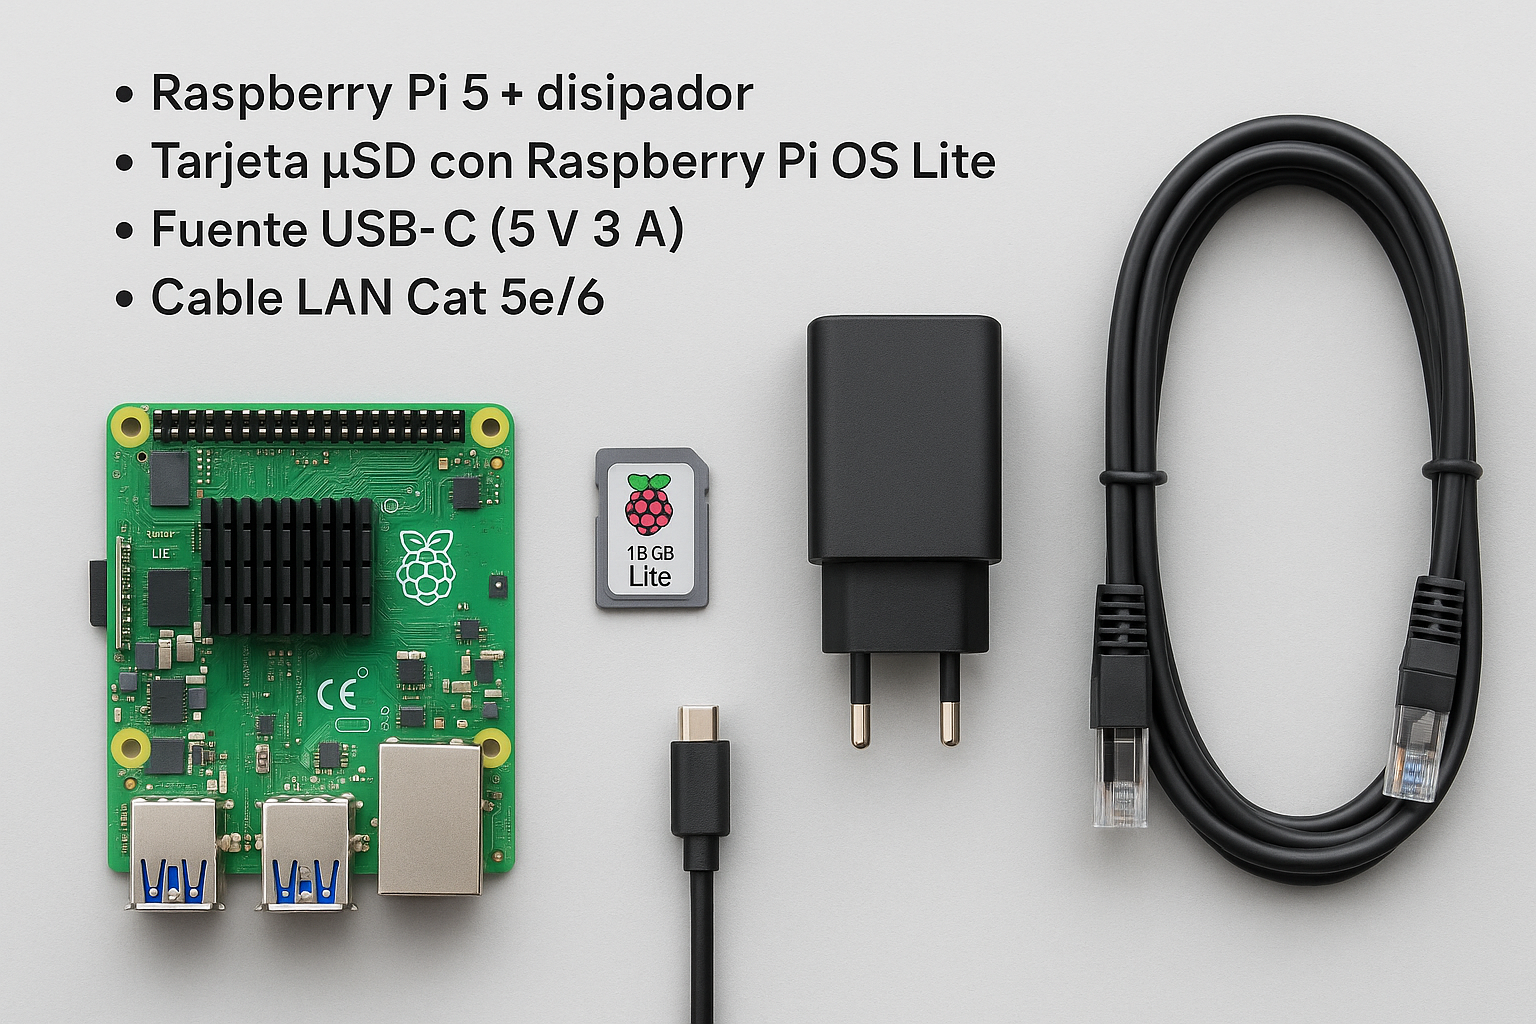
\includegraphics[width=\linewidth]{pi-implements.png}
    \end{column}
  \end{columns}
\end{frame}

%------------------------ cierre -----------------------------------
\begin{frame}%[standout]
  ¡Comencemos!\\
  \small Siguiente: encender la Pi y usar la terminal
\end{frame}

\end{document}

